\documentclass{article}
%
%
%	functional_analysis.tex
%
%	David Meyer
%	dmm613@gmail.com
%	02 Sep 2022
%
%
%   get various packages
%
\usepackage[margin=1.0in]{geometry}                                     % adjust margins
\geometry{letterpaper}                                                  % or a4paper or a5paper or ... 
\usepackage{url}                                                        % need this to use URLs in bibtex
\usepackage{setspace}                                                   % need this for \setstrech{...}
\usepackage{scrextend}                                                  % need this for addmargin
\usepackage[export]{adjustbox}                                          % need this to get frame for includegraphics
%
%   tikz et al
%
\usepackage{tikz}
\usetikzlibrary{calc,patterns,angles,quotes,shapes,math,decorations,
                through,intersections,lindenmayersystems,backgrounds,
                hobby}
\usepackage{circuitikz}                                                 % draw circuits    
\usepackage{pgfplots}
%
%	more math stuff
%
\usepackage{amsmath,amsfonts,amssymb,amsthm}
\usepackage{mathtools}
\usepackage{commath}                                                    % get \norm{x}
\usepackage{fixmath}                                                    % get \mathbold
\usepackage{gensymb}                                                    % get \degree
\usepackage{mathrsfs}
\usepackage{hyperref}
\usepackage{subcaption}
\usepackage{authblk}
\usepackage{graphicx}
\usepackage{hyperref}
\usepackage{alltt}
\usepackage{color}
\usepackage{float}
\usepackage{braket}
\usepackage{siunitx}
\usepackage{relsize}
\usepackage{multirow}
\usepackage{esvect}
%
%	watermarks
%
% \usepackage{draftwatermark}
% \SetWatermarkText{Draft}
% \SetWatermarkScale{5}
% \SetWatermarkLightness {0.9} 
% \SetWatermarkColor[rgb]{0.7,0,0}
%
%
%	theorems, definitions, etc
%
\theoremstyle{definition}
\newtheorem{theorem}{Theorem}[section]
\newtheorem{definition}{Definition}[section]
\newtheorem{proposition}{Proposition}[section]
\newtheorem{lemma}{Lemma}[section]
\newtheorem{example}{Example}[section]
\newtheorem{remark}{Remark}[section]
%
%	The following code allows you to do
%
%	\begin{bmatrix}[r] (or [c] or [l])
%
\makeatletter
\renewcommand*\env@matrix[1][c]{\hskip -\arraycolsep
  \let\@ifnextchar\new@ifnextchar
  \array{*\c@MaxMatrixCols #1}}
\makeatother
%
%	make \arg{min,max}_{n \to \infty} work nicely
%
\newcommand{\argmax}{\operatornamewithlimits{argmax}}
\newcommand{\argmin}{\operatornamewithlimits{argmin}}
%
%	handy commands
%
\newcommand*{\Scale}[2][4]{\scalebox{#1}{$#2$}}
\DeclareMathOperator{\E}{\mathbb{E}}
\DeclareMathOperator{\bda}{\Big \downarrow}						% big down arrow
\newcommand{\veq}{\mathrel{\rotatebox{90}{$=$}}}

%
%	Title, author and date
%
\title{A Few Notes on Functional Analysis}
\author{David Meyer \\ 
	{\small \vspace{-2.75mm} \href{mailto:dmm613@gmail.com}{dmm613@gmail.com}}}
\date{Last Update: \today \\
	{\small \vspace{1.00mm} Initial Version: June 8, 2018}}
%
%
%
\begin{document}
\maketitle
%
%
%
\section{Introduction}
Functional Analysis is an interesting topic because, among other
reasons, it sits between infinite dimensional linear algebra and
real and complex analysis \cite{fa_mit}. The connection is the
norm $\norm{\mathbf{x}}$ of a vector space $X$. As we shall see,
if $(X,\norm{\cdot})$ is a \emph{normed space} then $(X,d)$ is a
\emph{metric space} with metric $d(\mathbf{x},\mathbf{y})
\coloneqq \norm{\mathbf{y}-\mathbf{x}} =
\norm{\mathbf{x}-\mathbf{y}}$. Moreover, if
$(X,\langle\cdot,\cdot\rangle)$ is an \emph{inner product
space}\footnote{For $\mathbf{x}, \mathbf{y} \in \mathbb{R}^{n}$
the inner product is given by $\langle \mathbf{x}, \mathbf{y}
\rangle := \sum\limits_{i = 1}^{n} x_i y_i$.}  then
$(X,\norm{\cdot})$ is a normed space with norm $\norm{\mathbf{x}}
\coloneqq \sqrt{\langle \mathbf{x},\mathbf{x}\rangle}$ and
consequently $(X,d)$ is a metric space with metric
$d(\mathbf{x},\mathbf{y}) = \norm{\mathbf{x}-\mathbf{y}} =
\sqrt{\langle
\mathbf{x}-\mathbf{y},\mathbf{x}-\mathbf{y}\rangle}$.

\bigskip
\noindent
A metric $d(\mathbf{x},\mathbf{y})$ induces a topology $\tau_d$
on a set $X$, where $\tau_d := \{A \subseteq X \mid \text{for
every $\mathbf{x} \in A$}$ there exists an $\epsilon$ such that
$B_{\epsilon}(\mathbf{x}) \subseteq A\}$ \footnote{
$B_{\epsilon}(\mathbf{x})$ is the open epsilon ball centered at
$\mathbf{x}$. See Figure \ref{fig:open_epsilon_ball}.}. That is,
$\tau_d$ is a collection of open subsets of $X$.  The pair
$(X,\tau_d)$ is called a \emph{topological space}.

\bigskip
\noindent
One quick thing is to notice is that as we go from metric to norm
to inner product we are adding structure to a set or vector
space.  More specifically

\begin{equation*}
\begin{array}{rclll}
\text{metric:}        & d(\mathbf{x},\mathbf{y})                   
		& \longrightarrow & \text{measures distances} \\
\text{norm:}          & \norm{\mathbf{x}}
		& \longrightarrow & \text{measures distances, lengths} \\
\text{inner product:} & \langle\mathbf{x},\mathbf{y}\rangle 
		& \longrightarrow & \text{measures distances, lengths and angles}
\end{array}
\end{equation*}


\bigskip
\noindent
If we consider an arbitrary set $X$ with no other structure we
can only tell if two points are equal. A metric adds structure to
$X$ which allows us to calculate the distance between any two
points $x,y \in X$. Similarly, a norm adds structure to a vector
space that allows us to calculate length (as well as distance and
equality).  An inner product adds the ability to calculate
angles, etc. Both the algebraic and geometric aspects of this
increasing structure are pretty interesting.

\section{Metric Spaces}
\label{sec:metric_spaces}
Metric spaces, along with vector spaces are among the most
fundamental objects in Functional Analysis \cite{metric_spaces}.
The setup we consider is that we have an arbitrary set $X$ and we
look at two points $x,y \in X$. What we would like to do is
measure the distance between $x$ and $y$ in $X$ as shown in
Figure \ref{fig:set}.

\bigskip
\noindent
To measure this distance we define a map $d: X \times X
\rightarrow [0,\infty)$, which we call a metric and which has the
following three properties:


\begin{equation*}
\begin{array}{llll}
1. & d(x,y) \geq 0 \text{ and } d(x,y) = 0 \Leftrightarrow x = y
                && \hspace{5em} \mathrel{\#} \text{this property is called \emph{positive definiteness}} \\
[8pt]
2. & d(x,y) = d(y,x)
                && \hspace{5em} \mathrel{\#} \text{this property is called \emph{symmetry}} \\
[8pt]
3. & d(x,y) \leq d(x,z) + d(z,y)
                && \hspace{5em} \mathrel{\#} \text{this property is called the \emph{triangle inequality}} 
\vspace{0.50cm}																			% put some space between the list and the footnote
\end{array}
\end{equation*}



%
%	open epsilon ball
%
\begin{figure}[H]
\centering
  \resizebox{0.48 \textwidth}{!} {                                                              % resize the tikzpicture if you like
  \tikzstyle{background rectangle}=[thin,draw=black]                                            % make the frame thinner (there must be an easier way to do this)
     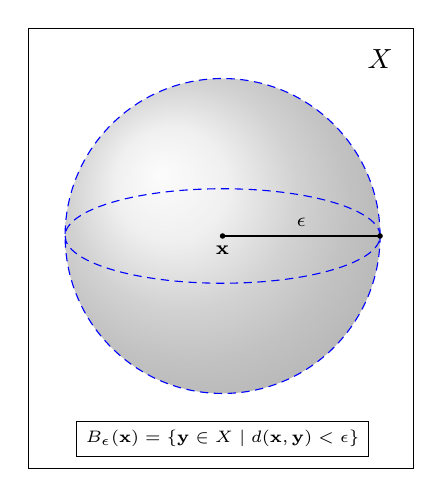
\begin{tikzpicture}[show background rectangle]                                             % couldn't control frame thickness with \begin{tikzpicture} [framed]
       \coordinate (C)  at (0.00, 0.00);                                                        % center
       \coordinate (R)  at (2.00, 0.00);                                                        % radius
       \coordinate (A)  at (-2.00,0.00);                                                        % arc (3D effect)
       \coordinate (RC) at (2.00, 2.25);                                                        % Right Corner (RC)
       \coordinate (S)  at (-2.20,2.25);                                                        % Spacing
       \shade [ball color = gray!40, opacity = 0.4] (0,0) circle (2cm);                         % draw the ball
       \draw  [densely dashed, draw=blue] (C) circle (2cm);                                     % draw the circle (use dashed because its an open ball)
       \draw  [densely dashed, draw=blue] (A) arc (180:360:2 and 0.6);                          % 3D effect
       \draw  [densely dashed, draw=blue] (R) arc (0:180:2 and 0.6);                            % draw the dashed line
       \fill  [fill=black] (C) circle (1pt);                                                    % draw a dot in the center
       \draw  [draw=none]  (C) node[font=\scriptsize, below] {$\mathbf{x}$};                    % label x
       \draw  [thin] (C) -- (R) node[font=\scriptsize,midway,above]{$\epsilon$};                % draw the radius (epsilon)
       \fill  [fill=black] (R) circle (1pt);                                                    % draw a dot at the edge
       \node  [] at  (RC) {$X$};                                                                % show X in the lower right corner
       \draw  [draw=none] (-2,-1.5) -- (2,-1.5)                                                 % draw the definition of the epsilon ball
				node[font=\fontsize{6.0}{1.0}\selectfont,rectangle, draw, very thin, below, midway, yshift=-0.85cm] 
				{$B_{\epsilon}(\mathbf{x}) =\{\mathbf{y} \in X \mid d(\mathbf{x},\mathbf{y}) < \epsilon\}$}; % defn of open epsilon ball
       \node  [] at (S) {};                                                                     % stretch out the frame so the ball is centered (Spacing)
     \end{tikzpicture}                                                                          % end tikzpicture
    }                                                                                           % end resizebox
    \caption{$B_{\epsilon}(\mathbf{x})$ is an open epsilon ball centered at $\mathbf{x}$ with radius $\epsilon$}
    \label{fig:open_epsilon_ball}
\end{figure}

\vspace{1.5em}
\noindent
We want the distance between $x$ and itself to be zero, hence
property 1. However, more than that we want this only to be the
case when $x = y$ (so if and only if). Of course we want the
distance from $x$ to $y$ to be the same as the distance from $y$
to $x$; this is property 2.  Finally, property 3, the triangle
inequality, is what we would expect in normal Euclidian space
\cite{euclidian_space}. The triangle inequality tells us that if
we take a "detour" through a third point $z$ then the distance
between $x$ and $y$ though $z$ will be greater than (or possibly
equal to) the distance between $x$ and $y$ on the direct path.
This is shown in Figure \ref{fig:triangle_inequality}. Note 
that there are important differences (which we will get to later) 
between distance, as measured by a metric $d(x,y)$ and length, 
as measured by a norm $\norm{\mathbf{x}}$, but for now we'll
consider the "distance version" of the triangle inequality as
shown in Figure \ref{fig:triangle_inequality}.

\vspace{2.5em}
\begin{figure}[H]
\centering
  \resizebox{0.55 \textwidth}{!} {	
    \tikzstyle{background rectangle}=[thin,draw=black]                                  % make the frame thinner (there must be an easier way) 
    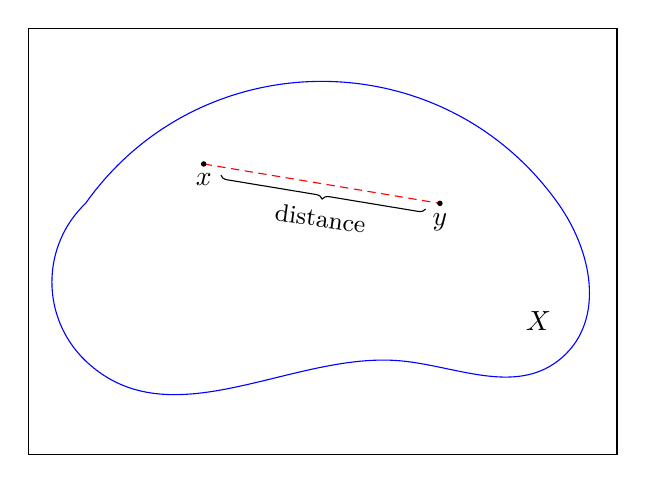
\begin{tikzpicture}[use Hobby shortcut, show background rectangle]                  % couldn't control thickness with \begin{tikzpicture} [framed]
%
%	\begin{tikzpicture}[use Hobby shortcut]
%														
%	coordinate system
%
		\coordinate (x)  at (1.50,-5.50);                                       % x endpoint of dashed line
		\coordinate (xb) at (1.80,-5.15);                                       % x endpoint of the brace
		\coordinate (y)  at (4.50,-6.00);                                       % y endpoint of the dashed line
		\coordinate (yb) at (4.40,-5.58);                                       % y endpoint of the brace					
		\coordinate (X)  at (5.75,-7.50);                                       % show X (the whole set) in lower right
%
%	draw everything
%
		\draw [draw=blue, rotate=-90, scale=2]                                  % draw the (blue) set boundary through these points
		       (3,0) .. +(1,0) .. +(1,2) .. +(1,3) .. +(0,3) .. (3,0);          % make the boundary go through these points
		\draw [] (x) node[below]{$x$};                                          % label x
		\draw [] (y) node[below]{$y$};                                          % label y
		\draw [densely dashed, draw=red] (x) -- (y);                            % draw the dashed line between x and y
		\draw [decoration={brace,mirror,raise=0.5cm},decorate] (xb) -- (yb)     % draw the underbrace
			node [rotate=-8.00,pos=0.5,anchor=north,yshift=-0.60cm] {${\small \text{distance}}$};   % label it with "distance"	
		\node [] at (X) {$X$};                                                  % draw X in the lower right corner
		\fill [fill=black] (x) circle (1.0pt);                                  % x dot
		\fill [fill=black] (y) circle (1.0pt);                                  % y dot
  \end{tikzpicture}                                                             % end tikzpicture
  }                                                                             % end resizebox
  \caption{The distance between $x$ and $y$ in $X$}
  \label{fig:set}
\end{figure}


\begin{figure}[b]
\centering
  \resizebox{0.55 \textwidth}{!} {	
    \tikzstyle{background rectangle}=[thin,draw=black]                                  % make the frame thinner (there must be an easier way) 
    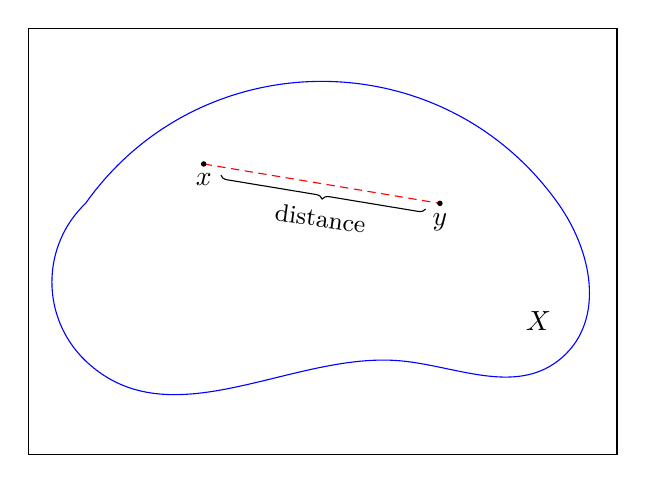
\begin{tikzpicture}[use Hobby shortcut, show background rectangle]                  % couldn't control thickness with \begin{tikzpicture} [framed]
%
%	\begin{tikzpicture}[use Hobby shortcut]
%														
%	coordinate system
%
		\coordinate (x)  at (1.50,-5.50);                                       % x endpoint of dashed line
		\coordinate (xb) at (1.80,-5.15);                                       % x endpoint of the brace
		\coordinate (y)  at (4.50,-6.00);                                       % y endpoint of the dashed line
		\coordinate (yb) at (4.40,-5.58);                                       % y endpoint of the brace					
		\coordinate (X)  at (5.75,-7.50);                                       % show X (the whole set) in lower right
%
%	draw everything
%
		\draw [draw=blue, rotate=-90, scale=2]                                  % draw the (blue) set boundary through these points
		       (3,0) .. +(1,0) .. +(1,2) .. +(1,3) .. +(0,3) .. (3,0);          % make the boundary go through these points
		\draw [] (x) node[below]{$x$};                                          % label x
		\draw [] (y) node[below]{$y$};                                          % label y
		\draw [densely dashed, draw=red] (x) -- (y);                            % draw the dashed line between x and y
		\draw [decoration={brace,mirror,raise=0.5cm},decorate] (xb) -- (yb)     % draw the underbrace
			node [rotate=-8.00,pos=0.5,anchor=north,yshift=-0.60cm] {${\small \text{distance}}$};   % label it with "distance"	
		\node [] at (X) {$X$};                                                  % draw X in the lower right corner
		\fill [fill=black] (x) circle (1.0pt);                                  % x dot
		\fill [fill=black] (y) circle (1.0pt);                                  % y dot
  \end{tikzpicture}                                                             % end tikzpicture
  }                                                                             % end resizebox
  \caption{The distance between $x$ and $y$ in $X$}
  \label{fig:set}
\end{figure}


%
%	triangle inequality
%
\begin{figure}[H]
\centering
  \resizebox{0.55 \textwidth}{!} {
    \tikzstyle{background rectangle}=[thin,draw=black]                                                          % make the frame thinner (there must be an easier way)
    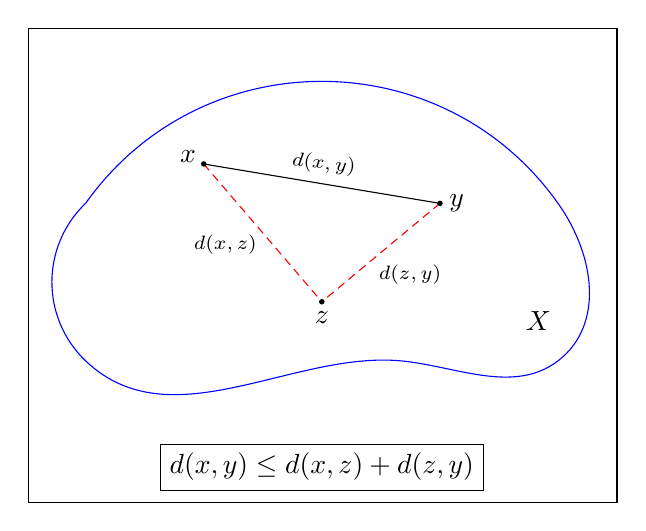
\begin{tikzpicture}[use Hobby shortcut, show background rectangle]                                          % couldn't control thickness with [framed]
%
%	\begin{tikzpicture}[use Hobby shortcut]
%														
%	coordinate system
%
		\coordinate (x)   at (1.50,-5.50);                                                              % x endpoint of dashed line
		\coordinate (xb)  at (1.80,-5.15);                                                              % x endpoint of the brace
		\coordinate (y)   at (4.50,-6.00);                                                              % y endpoint of the dashed line
		\coordinate (yb)  at (4.40,-5.58);                                                              % y endpoint of the brace
		\coordinate (z)   at (3.00,-7.25);                                                              % need a point z for the triangle inequality
		\coordinate (X)   at (5.75,-7.50);                                                              % show X (the whole set) in lower right
		\coordinate (TIL) at (2.25,-8.25);                                                              % left side of triangle inequality
		\coordinate (TIR) at (3.75,-8.25);                                                              % right side of triangle inequality

%
%	draw everything
%
		\draw [draw=blue, rotate=-90, scale=2]                                                          % draw the (blue) set boundary through these points
		       (3,0) .. +(1,0) .. +(1,2) .. +(1,3) .. +(0,3) .. (3,0);                                  % make the boundary go through these points
		\draw [] (x) node[left, above, , xshift=-2.00mm, yshift=-1.00mm]{$x$};                          % label x
		\draw [] (y) node[right, xshift=-0.05mm]{$y$};                                                  % label y
		\draw [] (z) node[below, yshift=-0.05mm]{$z$};                                                  % label z
		\draw [thin, draw=black] (x) -- (y)                                                             % draw x -- y
		       node[font=\scriptsize, rotate=-6.00, above, midway] {$d(x,y)$};                          % draw d(x,y)
		\draw [densely dashed, draw=red] (x) -- (z)                                                     % draw x -- z
		       node[font=\scriptsize, xshift=-4.75mm, yshift=1.00mm, below, midway] {$d(x,z)$};         % draw d(x,z)
		\draw [densely dashed, draw=red] (y) -- (z)                                                     % draw z -- y
		       node[font=\scriptsize, xshift=-1.50mm, yshift=-2.75mm, right, midway] {$d(z,y)$};        % draw d(z,y)
		\draw  [draw=none] (TIL) -- (TIR)                                                               % draw the definition of the triangle inequality
				node[rectangle, draw, very thin, below, midway, yshift=-0.80cm]                 % ...
				{$d(x,y) \leq d(x,z) + d(z,y)$};                                                % definition of the triangle inequality
		\fill [fill=black] (x) circle (1.0pt);                                                          % x dot		
		\fill [fill=black] (y) circle (1.0pt);                                                          % y dot
		\fill [fill=black] (z) circle (1.0pt);                                                          % z dot
		\node [] at (X) {$X$};                                                                          % draw X in the lower right corner
  \end{tikzpicture}                                                                                             % end tikzpicture
  }                                                                                                             % end resizebox
  \caption{The triangle inequality for distances}
  \label{fig:triangle_inequality}
\end{figure}
%
%
%
\bigskip
\section{Conclusions}
One way to look at the relationship between inner product, metric, normed, and 
topological spaces is shown in Figure \ref{figure:spaces}.

\bigskip

\renewcommand{\arraystretch}{1.00}
\setlength {\fboxrule}{0.75pt}							% set the outside \fcolorbox line thickness
\setlength {\fboxsep} {1.00em}							% get more space between \fcolorbox and content
%
%
%
\begin{figure}[H]										% build the figure
  \centering											% center everything
  \fcolorbox{black}{white} {								% make the frame blue
        \resizebox{1.0 \textwidth}{!} {
		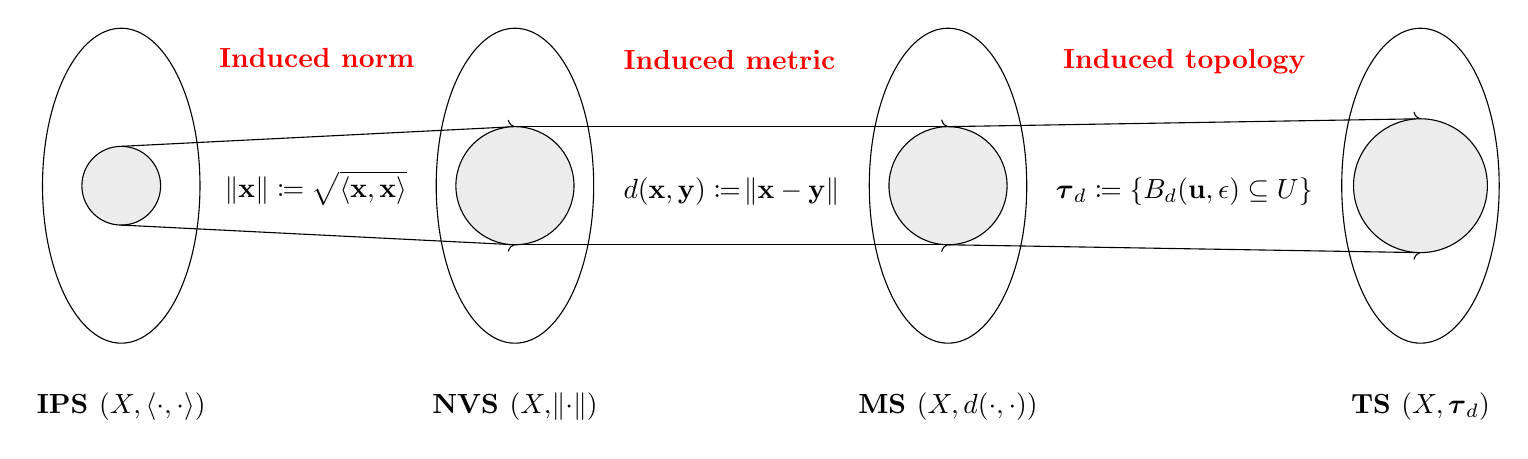
\begin{tikzpicture}
%
%
%
            \coordinate (O)    at (0.00,0.00);			% origin
            \coordinate (IPSs) at (0.00,0.50);			% IPS origin
            \coordinate (IPSd) at (5.0,0.75);			% IPS origin
%
%	Inner Product Spaces
%
			\draw (O) ellipse (1cm and 2cm) node [midway,below,yshift=-2.50cm] 
							{$\text{\bf IPS $(X,\langle \cdot,\cdot \rangle)$}$};	
			\draw[fill=gray!15] (O) circle (0.50) node [] {};
%
%	Normed Vector Spaces
%	
    		\draw [->] (IPSs) -- (IPSd) node [midway,above,xshift=-0.50,yshift=0.75cm] 
							{$\color{red}{\text{\bf Induced norm}}$};
		    \draw [draw=none] (IPSs) -- (IPSd) node [midway,above,xshift=-0.750,yshift=-3.750cm] {};
    		\draw [->] (0,-0.5) -- (5.0,-0.75);
    		\draw[draw=none] (3.5,0.50) -- (1.5,0.75) node [midway,above,yshift=-1.0cm] 
							{$\norm{\mathbf{x}} \coloneqq \sqrt{\langle {\mathbf x},{\mathbf x} \rangle}$};
    		\draw (5,0.0) ellipse (1cm and 2cm) node [midway,below,xshift=5.0cm,yshift=-2.50cm]
							{$\text{\bf NVS $(X,\norm{\cdot})$}$};
			\draw[fill=gray!15] (5.0,0) circle (0.750) node [] {};   

%
%	Metric Spaces
%	
    		\draw (10.50,0.0) ellipse (1cm and 2cm) node [midway,below,xshift=10.50cm,yshift=-2.5cm]
							{$\text{\bf MS $(X,d(\cdot,\cdot))$}$};	
    		\draw [->] (5,0.75) -- (10.50,0.75) node [midway,above,xshift=-0.75,yshift=0.60cm] 
							{$\color{red}{\text{\bf Induced metric}}$};
		    \draw [draw=none] (5,0.5) -- (10.0,0.75) node [midway,above,xshift=-0.50,yshift=-3.750cm] {};
    		\draw [->] (5,-0.75) -- (10.50,-0.75);
    		\draw[fill=gray!15] (10.50,0) circle (0.750) node [] {};
		    \draw[draw=none] (5,0.50) -- (10.50,0.75) node [midway,above,yshift=-1.0cm] 
		    				{$d(\mathbf{x},\mathbf{y}) \coloneqq \norm{\mathbf{x}-\mathbf{y}}$};
 
%
%	Topological spaces
%  
			\draw (16.5,0.0) ellipse (1cm and 2cm) node [midway,below,xshift=16.5cm,yshift=-2.5cm]
							{$\text{\bf TS $(X,{\boldsymbol \tau_{d}})$}$};	
			\draw [->] (10.50,0.75) -- (16.5,0.85) node [midway,above,yshift=0.50cm] 
							{$\color{red}{\text{\bf Induced topology}}$};
			\draw [draw=none] (10,0.5) -- (16.5,0.75) node [midway,above,xshift=0.50cm,yshift=-3.750cm] {};
			\draw [->] (10.50,-0.75) -- (16.5,-0.85);
			\draw[fill=gray!15] (16.5,0) circle (0.85) node [] {};   
			\draw[draw=none] (10.50,0.50) -- (16.5,0.75) node [midway,above,yshift=-1.0cm] 
						{${\boldsymbol \tau_d} \coloneqq \{B_{d}(\mathbf{u},\epsilon) \subseteq U\}$};
		\end{tikzpicture}
		}
	}
	\caption{Induced Norm, Metric, and Topology}
	\label{figure:spaces}
\end{figure}

\bigskip
\setlength {\fboxsep} {0.50em}							% get more space between \fcolorbox and content
\setlength {\fboxrule}{0.75pt}							% set the outside \fcolorbox line thickness
\begin{figure}[H]										% build the figure
  \centering											% center everything
  \fcolorbox{black}{gray!5} {							% make the outside frame black
	 \resizebox{1.00\textwidth}{!} {
	    \begin{math}
          \begin{array}{llllll}
            {\bf IPS} &--& \text{Inner Product Spaces}	&&	(X,\langle {\bf x},{\bf y} \rangle)\\
            {\bf NVS} &--& \text{Normed Vector Spaces}	&&	(X,\norm{\bf x}) = (X,\sqrt{\langle \bf {x}, \bf{x}} \rangle) \\
            {\bf MS}  &--& \text{Metric Spaces}			&&	(X,d({\bf x},{\bf y})) = (X, \norm{{\bf x} - {\bf y}}) = 
                                                			(X,\sqrt{\langle {\bf x} - {\bf y},{\bf x} - {\bf y}}\rangle)\\
            {\bf TS}  &--& \text{Topological Spaces}	&&	(X, {\boldsymbol \tau_d)}, \text{ where ${\boldsymbol \tau_d = }$ 
            												\{open subsets of $(X, d)$\}}
           \end{array}
        \end{math}
     }
  }
\end{figure}
%
%
%
\bigskip
\section*{Acknowledgements}
%
%	LaTeX source on overleaf.com
%
\section*{\LaTeX \hspace{0.10 mm} Source}
\url{https://www.overleaf.com/read/fgrrxmkycvry}
%
%	get a bibliography
%
%	Note:.bib files go in ~/Library/texmf/bibtex/bib with TeXShop (MacTeX).
%	You can also use an absolute path, e.g. \bibliography{/Users/dmm/papers/bib/qc}
%
\bibliographystyle{plain}
\bibliography{qc}
%
%	done
%
\end{document} 


